%!BIB TS-program = biber
\documentclass[11pt]{article}%
\usepackage{amsmath}
\usepackage{amsfonts}
\usepackage{amssymb,tcolorbox}
\usepackage{graphicx}
\usepackage{amssymb}%
\usepackage{siunitx}
\usepackage{listings}
\usepackage[style=ieee]{biblatex}
\setcounter{MaxMatrixCols}{30}
\providecommand{\U}[1]{\protect\rule{.1in}{.1in}}
\providecommand{\U}[1]{\protect\rule{.1in}{.1in}}
\providecommand{\U}[1]{\protect\rule{.1in}{.1in}}
\newtheorem{theorem}{Theorem}
\newtheorem{acknowledgement}[theorem]{Acknowledgement}
\newtheorem{algorithm}[theorem]{Algorithm}
\newtheorem{axiom}[theorem]{Axiom}
\newtheorem{case}[theorem]{Case}
\newtheorem{claim}[theorem]{Claim}
\newtheorem{conclusion}[theorem]{Conclusion}
\newtheorem{condition}[theorem]{Condition}
\newtheorem{conjecture}[theorem]{Conjecture}
\newtheorem{corollary}[theorem]{Corollary}
\newtheorem{criterion}[theorem]{Criterion}
\newtheorem{definition}[theorem]{Definition}
\newtheorem{example}[theorem]{Example}
\newtheorem{exercise}[theorem]{Exercise}
\newtheorem{lemma}[theorem]{Lemma}
\newtheorem{notation}[theorem]{Notation}
\newtheorem{problem}[theorem]{Problem}
\newtheorem{proposition}[theorem]{Proposition}
\newtheorem{remark}[theorem]{Remark}
\newtheorem{solution}[theorem]{Solution}
\newtheorem{summary}[theorem]{Summary}
\newenvironment{proof}[1][Proof]{\noindent\textbf{#1.} }{\ \rule{0.5em}{0.5em}}
\addtolength{\oddsidemargin}{-.875in}
\addtolength{\evensidemargin}{-.875in}
\addtolength{\textwidth}{1.75in}
\addtolength{\topmargin}{-1in}
\addtolength{\textheight}{2in}
\usepackage{tocloft}
\usepackage{color} %red, green, blue, yellow, cyan, magenta, black, white
\definecolor{mygreen}{RGB}{28,172,0} % color values Red, Green, Blue
\definecolor{mylilas}{RGB}{170,55,241}

\addbibresource{proj5.bib}

\title{MANE 6710 - Numerical Design Optimization Lab 5}
\author{Human 6966}
\date{December 18 2024}

\renewcommand{\contentsname}{Table of Contents:}
\setcounter{tocdepth}{3} % Include sections and subsections
\setlength{\cftbeforesecskip}{0.5cm} % Adjust spacing between entries
\begin{document}
\maketitle
\newpage
\tableofcontents
\newpage
\addcontentsline{toc}{section}{Executive Summery}
\section*{Executive Summery}
\label{sec:abstract}

Unconstrained optimization algorithms are powerful tools for engineers, as they form a basic method of solving complex multivariable optimization problems found across engineering disciplines. The purpose of this lab was for us to implement  an unconstrained optimization problem from scratch to learn more about how they work. The algorithm I implemented was the Broyden–Fletcher–Goldfarb–Shanno algorithm, which is a nonlinear multivariable Quasi-Newton algorithm, that is relatively efficient for medium to large smooth optimization problems. I was successfully able to implement this algorithm in Python, which runs with reasonable efficiency and accuracy.

\section{Introduction}
\label{sec:intro}

Optimization algorithms are an important tool for engineers as they enable us to numerically determine a viable solution to a complex problem that balances various design criteria (such as weight, cost, or strength). Optimization algorithms  solve these problems by numerically solving a given input equation set (called the objective function) for a local minimum. These algorithms use various methods to solve for these local minimums, which have different strengths and weaknesses. 

For example, genetic algorithms can solve nonlinear equations that have a discontinuous first derivative as it rellies solly on the objective function. However, the downside of this paticular method is its computational cost as sampling the objective function several times each iteration to determine the best movement diretion takes more time and power than other methods like the Broyden–Fletcher–Goldfarb–Shanno algorithm (BFGS). 

The BFGS algorithm is a non-linear Quasi-Newton optimization algorithm that is significantly more efficient than the genetic algorithm. This is because it uses derivative and approximated second derivative information to reduce the number of function calls and iterations used to determine a local minimum. However, the downside to using this and other Quasi-Newton methods is they rely on the function having a continuous, easily computed first derivative. This means that there are problems the genetic algorithm is capable of solving that the BFGS algorithm cannot.

\section {Methodology}
\label{sec:method}

The BFGS algorithm I implemented in this project is from algorithms 6.1, 3.5, and 3.6 \cite{textbook} shown in Figures \ref{fig:bfgsmethod}, \ref{fig:bfgsline}, and \ref{fig:bfgszoom} respectively.
\begin{figure}[!ht]
    \centering
   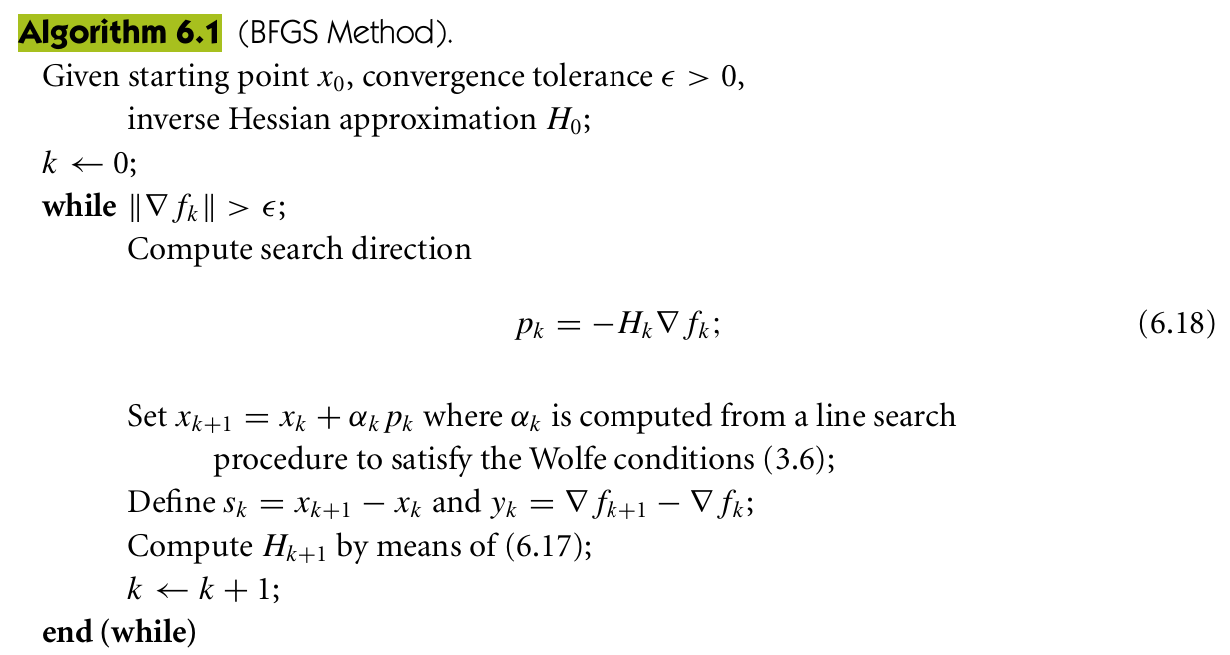
\includegraphics[width=0.75\linewidth]{al61.png}
    \caption{Algorithm 6.1: BFGS Method }
   \label{fig:bfgsmethod}
\end{figure}
\begin{figure}[!ht]
    \centering
   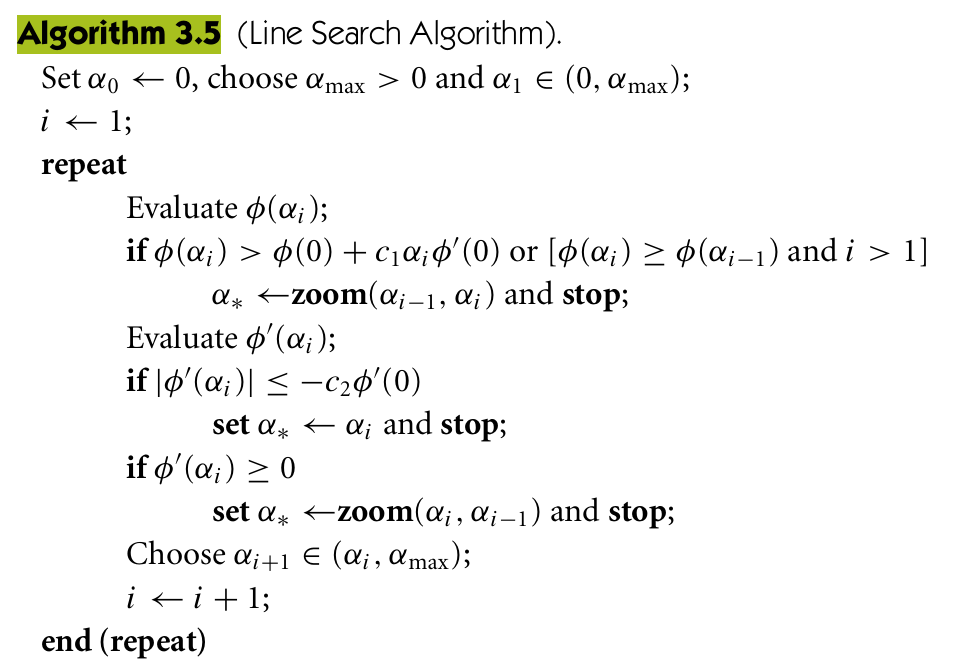
\includegraphics[width=0.75\linewidth]{al35.png}
    \caption{Algorithm 3.5: BFGS Line Search Method }
   \label{fig:bfgsline}
\end{figure}
\begin{figure}[!ht]
    \centering
   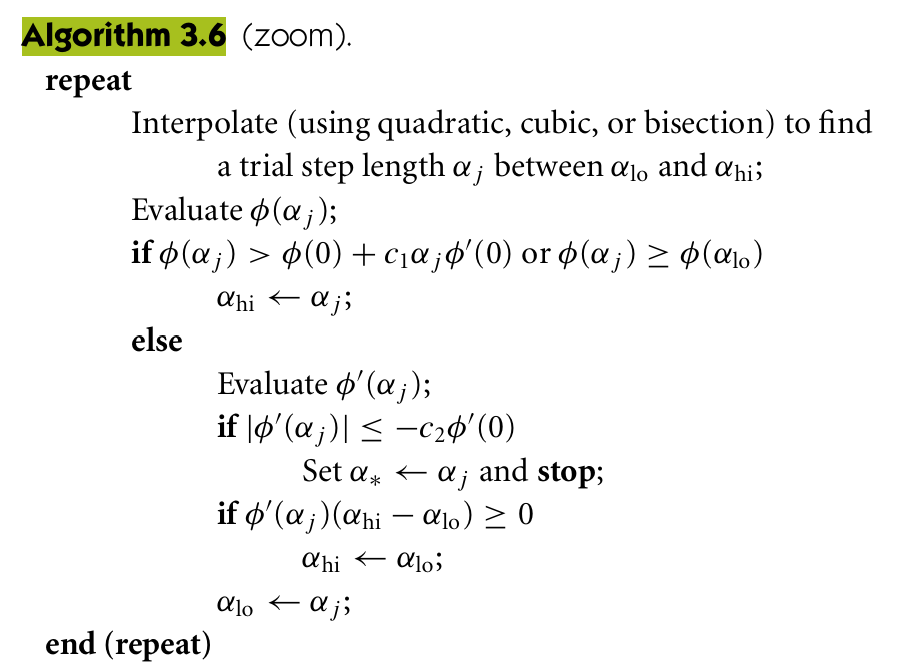
\includegraphics[width=0.75\linewidth]{al36.png}
    \caption{Algorithm 3.6: BFGS Zoom Method }
   \label{fig:bfgszoom}
\end{figure}

My implementation of this algorithm works by using the complex step method to calculate the gradient ($\nabla f_{k}$) at the current position ($x_{k}$) using a step size of $10^{-30}$. Then my code calculates the step direction ($p_{k}$) from the gradient and the current approximation of the hessian ($H_{k}$) using the equation $p_{k}=-H_{k}\nabla f_{k}$. From this and the given objective function ($f(x)$), an anonymous scalar function is defined as $\phi(\alpha)=f(x_{k}+\alpha p_{k})$ and an anonymous function for the derivative is defined as $\phi'(\alpha)=\nabla \phi(\alpha)$, which are given to the line search algorithm to solve for a minimum in the search direction.

The Line Search algorithm iterates through values of $\alpha$ until it either finds values on both sides of the directional minimum, finds an increasingly positive first derivative, or runs out of allowed iterations. In the first case, the line search method calls the Zoom algorithm, passing it the two endpoints and the scalar functions, and returns its output. In the second case, the function returns the current value of $\alpha$ and in the third case the algorithm throws a runtime error.

The Zoom algorithm performs a bisection search on the given interval of the scalar function, checking if the current $\alpha$ satisfies the strong Wolfe conditions for each iteration. When the strong Wolfe conditions are satisfied, the algorithm returns the current step length ($\alpha_{\text{current step}}=0.5(\alpha_{\text{high bound}}+\alpha_{\text{low bound}})$). In iterations where the strong Wolf conditions aren't met, the algorithm sets the high bound of the interval to the current step if the sufficient decrease condition ($\phi(\alpha_{\text{current step}})<\phi(0)+c_{1}\alpha_{\text{current step}}\phi'(0)$) isn't satisfied and the low bound of the interval to the current step if the sufficient decrease condition is met but the flatness condition ($|\phi'(.\alpha_{\text{current step}})|\leq -c_{2}\phi'(0)$). Note: $c_1$ and $c_2$ were chosen to be 0.0001 and 0.9 respectively based on the advice from the textbook \cite{textbook}.

Once the Zoom and Line Search algorithms return the current step length ($\alpha$), the BFGS algorithm updates the current position, gradient, and Hessian estimate. The Hessian estimate update equation is given in Equation \ref{eqn:hessupdate} \cite{textbook} ( $y_{k}$, and $s_{k}$, and $\rho_{k}$ are given in Equations \ref{eqn:yk},  \ref{eqn:sk}, and \ref{eqn:rhok} respectively). Then the current step statistics are printed to the terminal and the ending condition ($||\nabla f(x_{k})||<\text{Error Tolerance}$) is checked to determine if the algorithm needs another iteration and, if not, returns the final position.
\begin{equation}
\label{eqn:hessupdate}
H_{k+1}= (I-\rho_{k}s_{k}y_{k}^{T})H_{k}(I-\rho_{k}y_{k}s_{k}^{T})+\rho_{k}s_{k}s_{k}^{T}
\end{equation}
\begin{equation}
\label{eqn:yk}
y_{k}=\nabla f(x_{k+1})-\nabla f(x_{k})
\end{equation}
\begin{equation}
\label{eqn:sk}
s_{k}=\alpha p_{k}
\end{equation}
\begin{equation}
\label{eqn:rhok}
\rho_{k}=\frac{1}{y_{k}^{T}s_{k}}
\end{equation}

\section{Testing and Results}

Once I implemented the algorithm in Python, the algorithm needed to be tested to ensure it worked. The test cases and the algorithm's results are summarized in Table \ref{table:cases}. I chose a scalar function for the first test case, as it is a special case that isn't affected by matrix algebra errors while still testing the different algorithms and their integration. Once I ensured the algorithm was running as intended with the scalar case, I chose to implement two simple two-dimensional polynomial cases to test the matrix algebra implementation and how the code handles vectors. There were several matrix algebra errors due to how the Numpy library handles arrays that were fixed using these test cases. The final set of test cases I chose to test the algorithm's ability to handle more complex problems. The Two-dimensional Rosenbrock function was suggested by the instructor as a good single-objective optimization test case used in research. The fifth test case tested how the algorithms reacted to multimodal cases and the sixth tested the algorithm's ability to handle higher dimensional problems. See Table \ref{table:initial} for the initial conditions used in each test case.
\begin{table}[!ht]
\caption{Test Cases and Algorithm Results}
\label{table:cases}
\begin{tabular}{llll}
Test Case                                                                & Actual Minima Location     & Calculated Minima Location & Apendix \\ \hline
$x^2$                                                                       & 0                  & 0,0             & \ref{sec:onedpoly}     \\
$x_1^4 + x_2^2   $                                                             & (0,0)              & (1.28e-3,-2.10e-8),(1.28e-3,-2.10e-8)                & \ref{sec:twodpoly}     \\
$(x_1-1)^4+(x_2+2)^2$                                          & (1,-2)             & (0.999,-1.9999), (1.001,-1.99999)  &    \ref{sec:twodpolyshift}     \\
two dimensional Rosenbrock                                               & (1,1)              &    (1,1)               &   \ref{sec:rosbrock}      \\
$x_1^4 + x_2^4 - 17x_2^3 +45 x_2^2$     & (1,3), (1,13.6342) & (1.0002,3),(0.9972,13.6342)  &     \ref{sec:twodpolymult}    \\
$(x_1-1)^4+(x_2+2)^2+1+5(x_3-3)^4 $              & (1,-2,3)           & (0.9996,-2,3), (1.0015,-2,3)    &        \ref{sec:threedpoly}
\end{tabular}
\end{table}

\begin{table}[!ht]
\center
\caption{Initial Conditions for Test Cases}
\label{table:initial}
\begin{tabular}{lll}
Test Case                                                                & $x_0$                 & $H_0$    \\ \hline
$x^2$                                                                       & 10,-10                  & $0.1I$    \\
$x_1^4 + x_2^2   $                                                             & (10,10),(-10,-10)              &$0.1I$     \\
$(x_1-1)^4+(x_2+2)^2$                                          & (4,4),(-7,-7)             & $0.05I$ \\
two dimensional Rosenbrock                                               & (1,1)              &    $0.1I$ \\
$x_1^4 + x_2^4 - 17x_2^3 +45 x_2^2$     & (4,4),(-7,-7) & $0.1I$   \\
$(x_1-1)^4+(x_2+2)^2+1+5(x_3-3)^4 $              & (4,4,4),(-7,-7,-7)   & $0.1I$
\end{tabular}
\end{table}

As is shown in Table \ref{table:cases}, the algorithm I implemented was able to consistently find a minimum within a reasonable time frame (the largest number of iterations used being 34 in the used test cases). While there is some error between the calculated and actual minima locations, particularly in cases with unequal scaling. As shown in the Appendix section for each test case, the First-order Optimality (magnitude of the gradient) decreased by at least nine orders of magnitude demonstrating a properly functioning optimization algorithm converging on a viable solution. Between the low error in the results and the convergence history, my implementation of the BFGS algorithm is shown to work in all of the test cases.


\medskip


\section{Conclusions}

I was able to successfully implement the nonlinear unconstrained optimization algorithm BFGS. As shown in the results, the implemented algorithm was able to handle simple and complex smooth nonlinear multivariable optimization problems efficiently. However, my implementation of the BFGS algorithm has significant limitations. Firstly, it only handles unconstrained optimization algorithms. This limits the potential applications for this algorithm as most problems in engineering have constraints. This can be somewhat mitigated by adding barrier functions to the objective function, however, it will likely be less efficient and accurate than an algorithm designed for handling constraints. Secondly, the algorithm only works with deterministic functions that are 'smooth' and have a continuous first derivative. Thirdly, this implementation is less efficient for linear optimization problems than purpose-made algorithms. Finally, this algorithm doesn't handle functions that go to negative infinity well (it usually throws an error), so it should only be used on functions with real minima.

\addcontentsline{toc}{section}{References}
\printbibliography
\newpage
\section{Appendix}

\subsection{Optimization Algorithm Test Case Output}

\subsubsection{One Dimentional Polynomial}
\label{sec:onedpoly}
\begin{figure}[!ht]
    \centering
   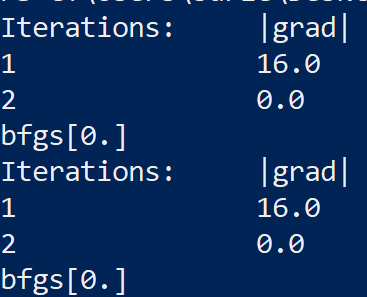
\includegraphics[width=0.75\linewidth]{oned.png}
    \caption{Function output for one dimensional polynomial from two starting points}
    \label{fig:onedpoly}
\end{figure}
\newpage
\subsubsection{Two Dimentional Polynomial}
\label{sec:twodpoly}
\begin{figure}[!ht]
    \centering
   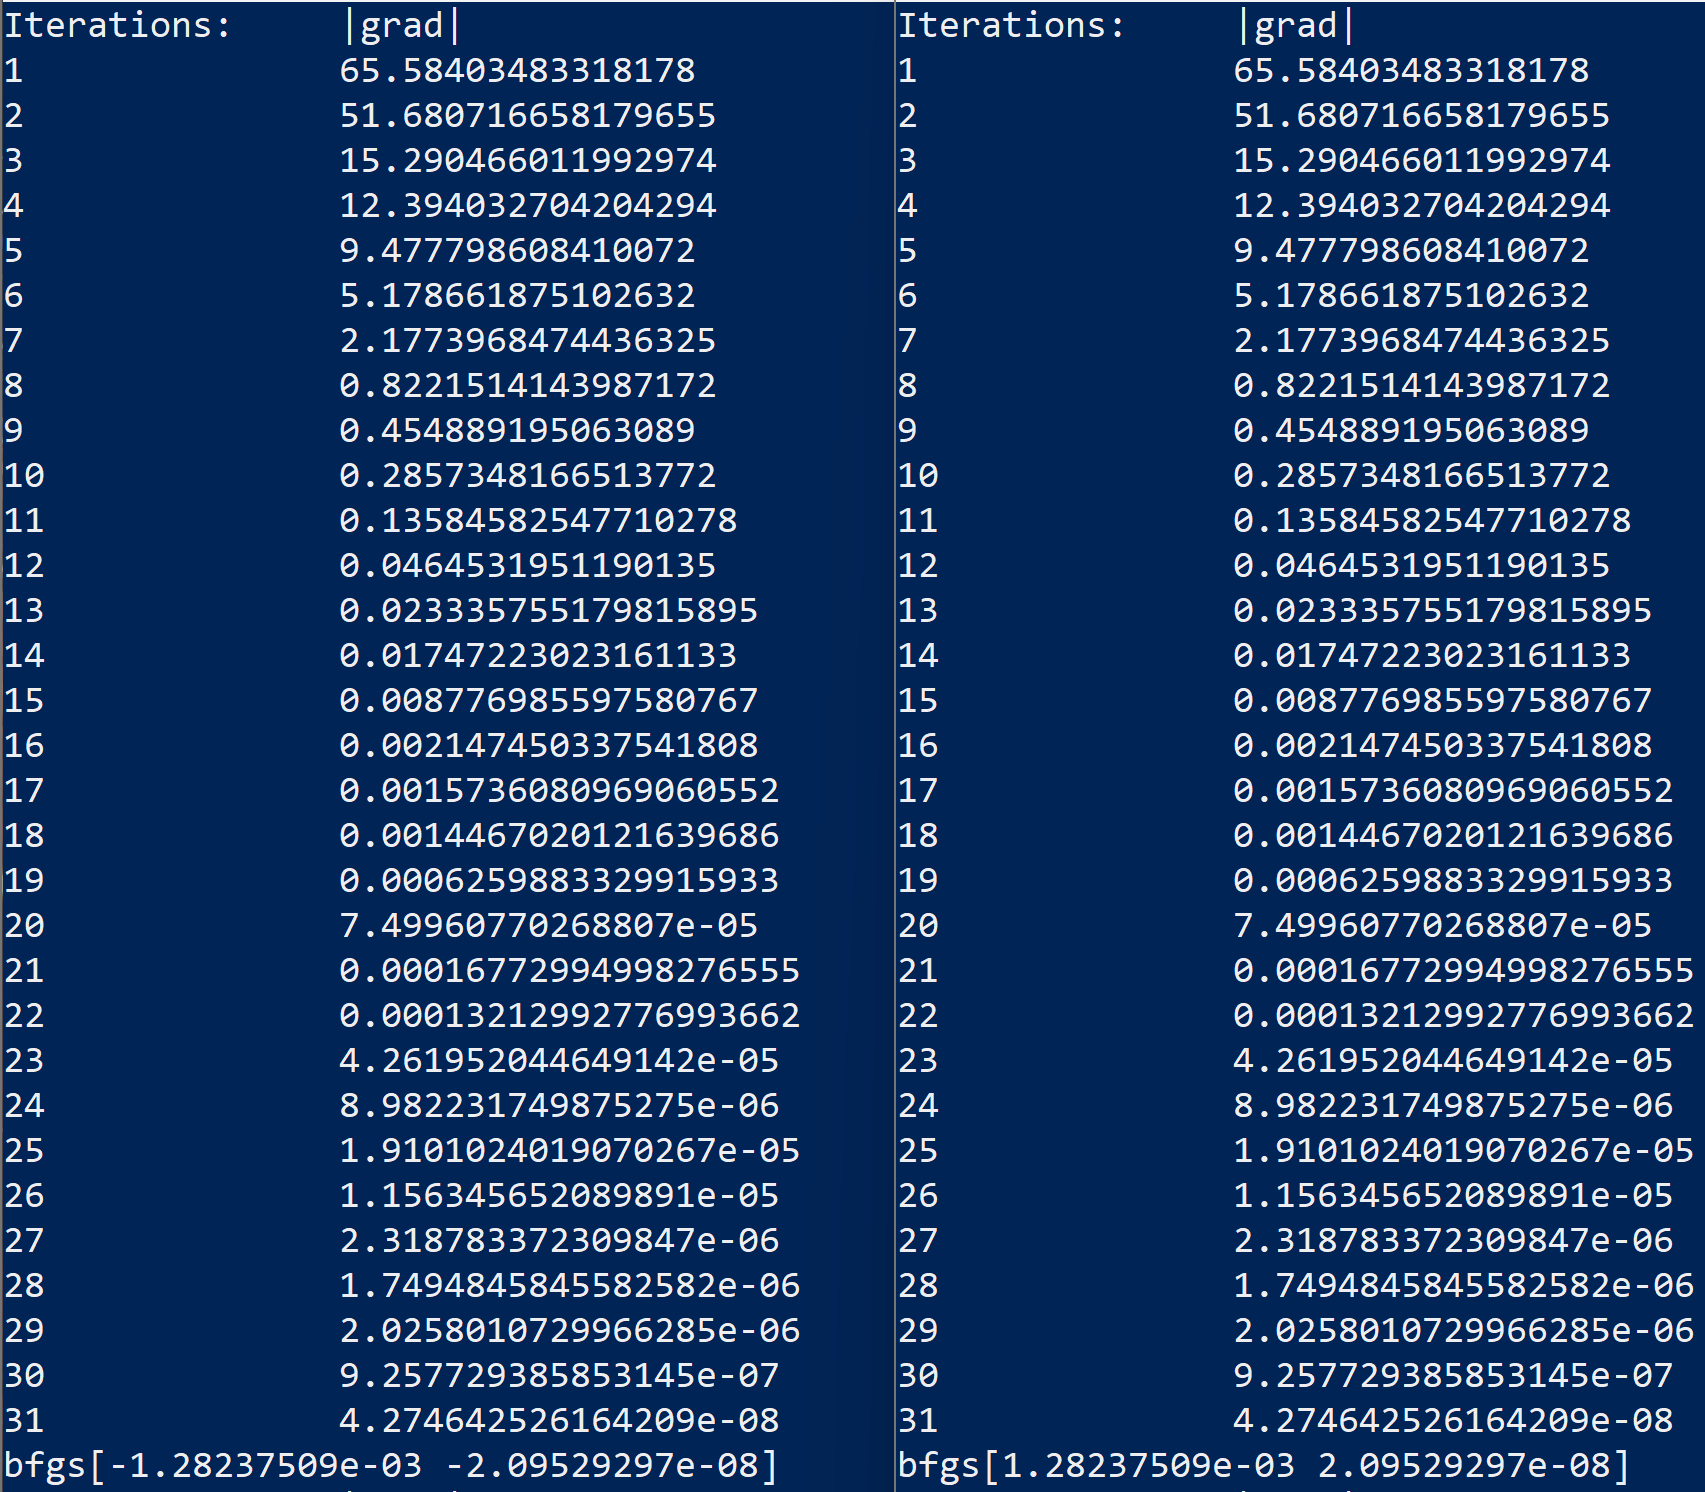
\includegraphics[width=0.75\linewidth]{d2.png}
    \caption{Function output for two dimensional polynomial from two starting points}
    \label{fig:d2}
\end{figure}
\newpage
\subsubsection{Shifted Two Dimentional Polynomial}
\label{sec:twodpolyshift}
\begin{figure}[!ht]
    \centering
   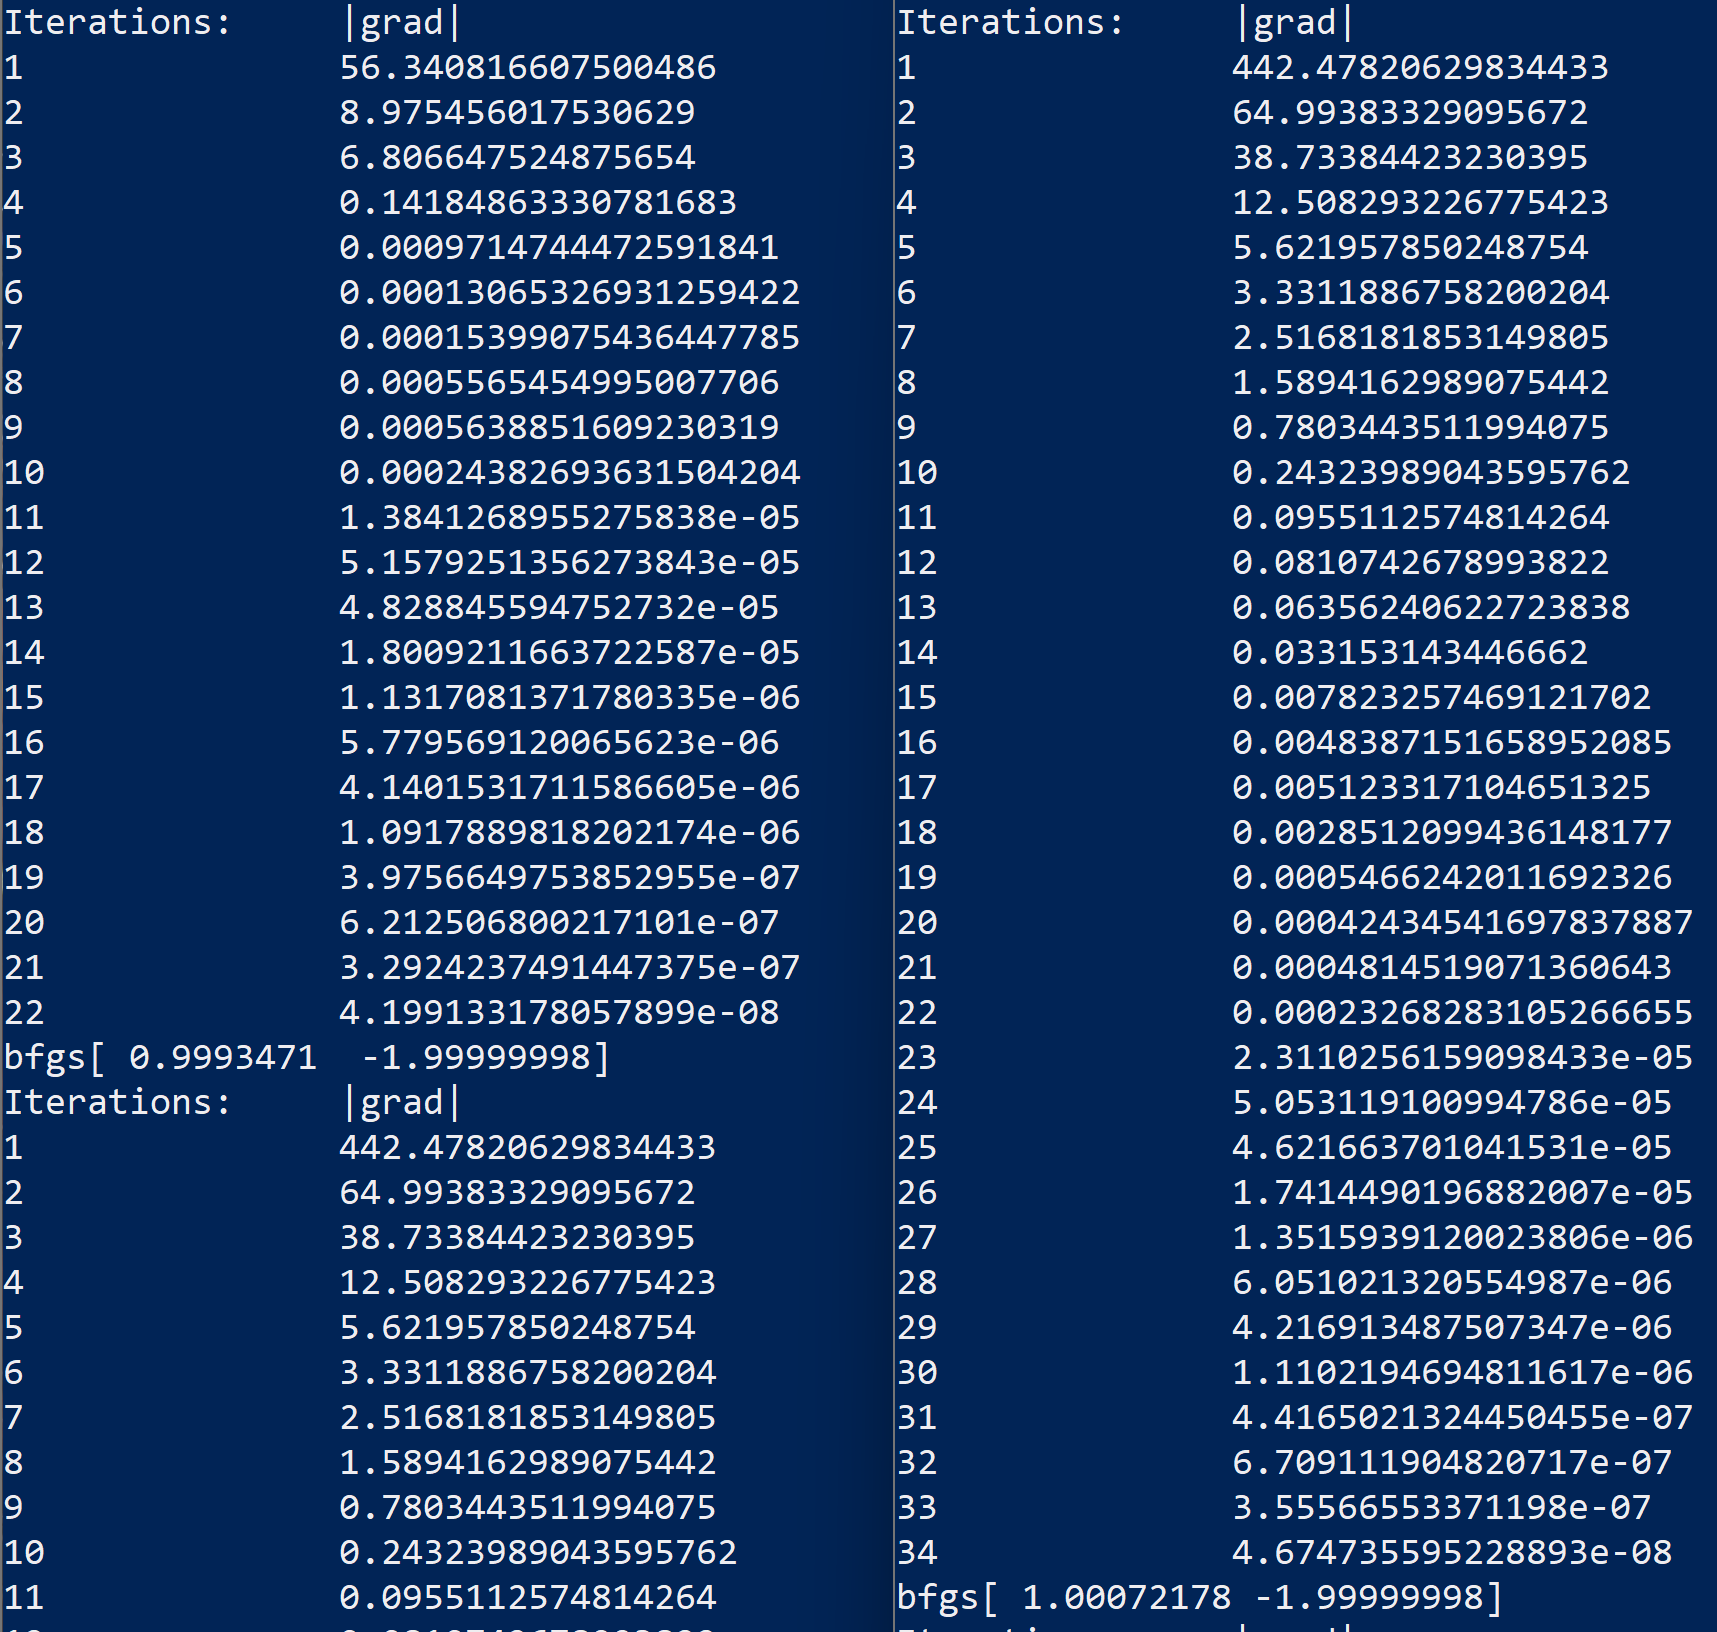
\includegraphics[width=0.75\linewidth]{d2shifted.png}
    \caption{Function output for two dimensional polynomial from two starting points}
    \label{fig:d2shifted}
\end{figure}
\newpage
\subsubsection{Two Dimentional Rosenbrock Function}
\label{sec:rosbrock}
\begin{figure}[!ht]
    \centering
   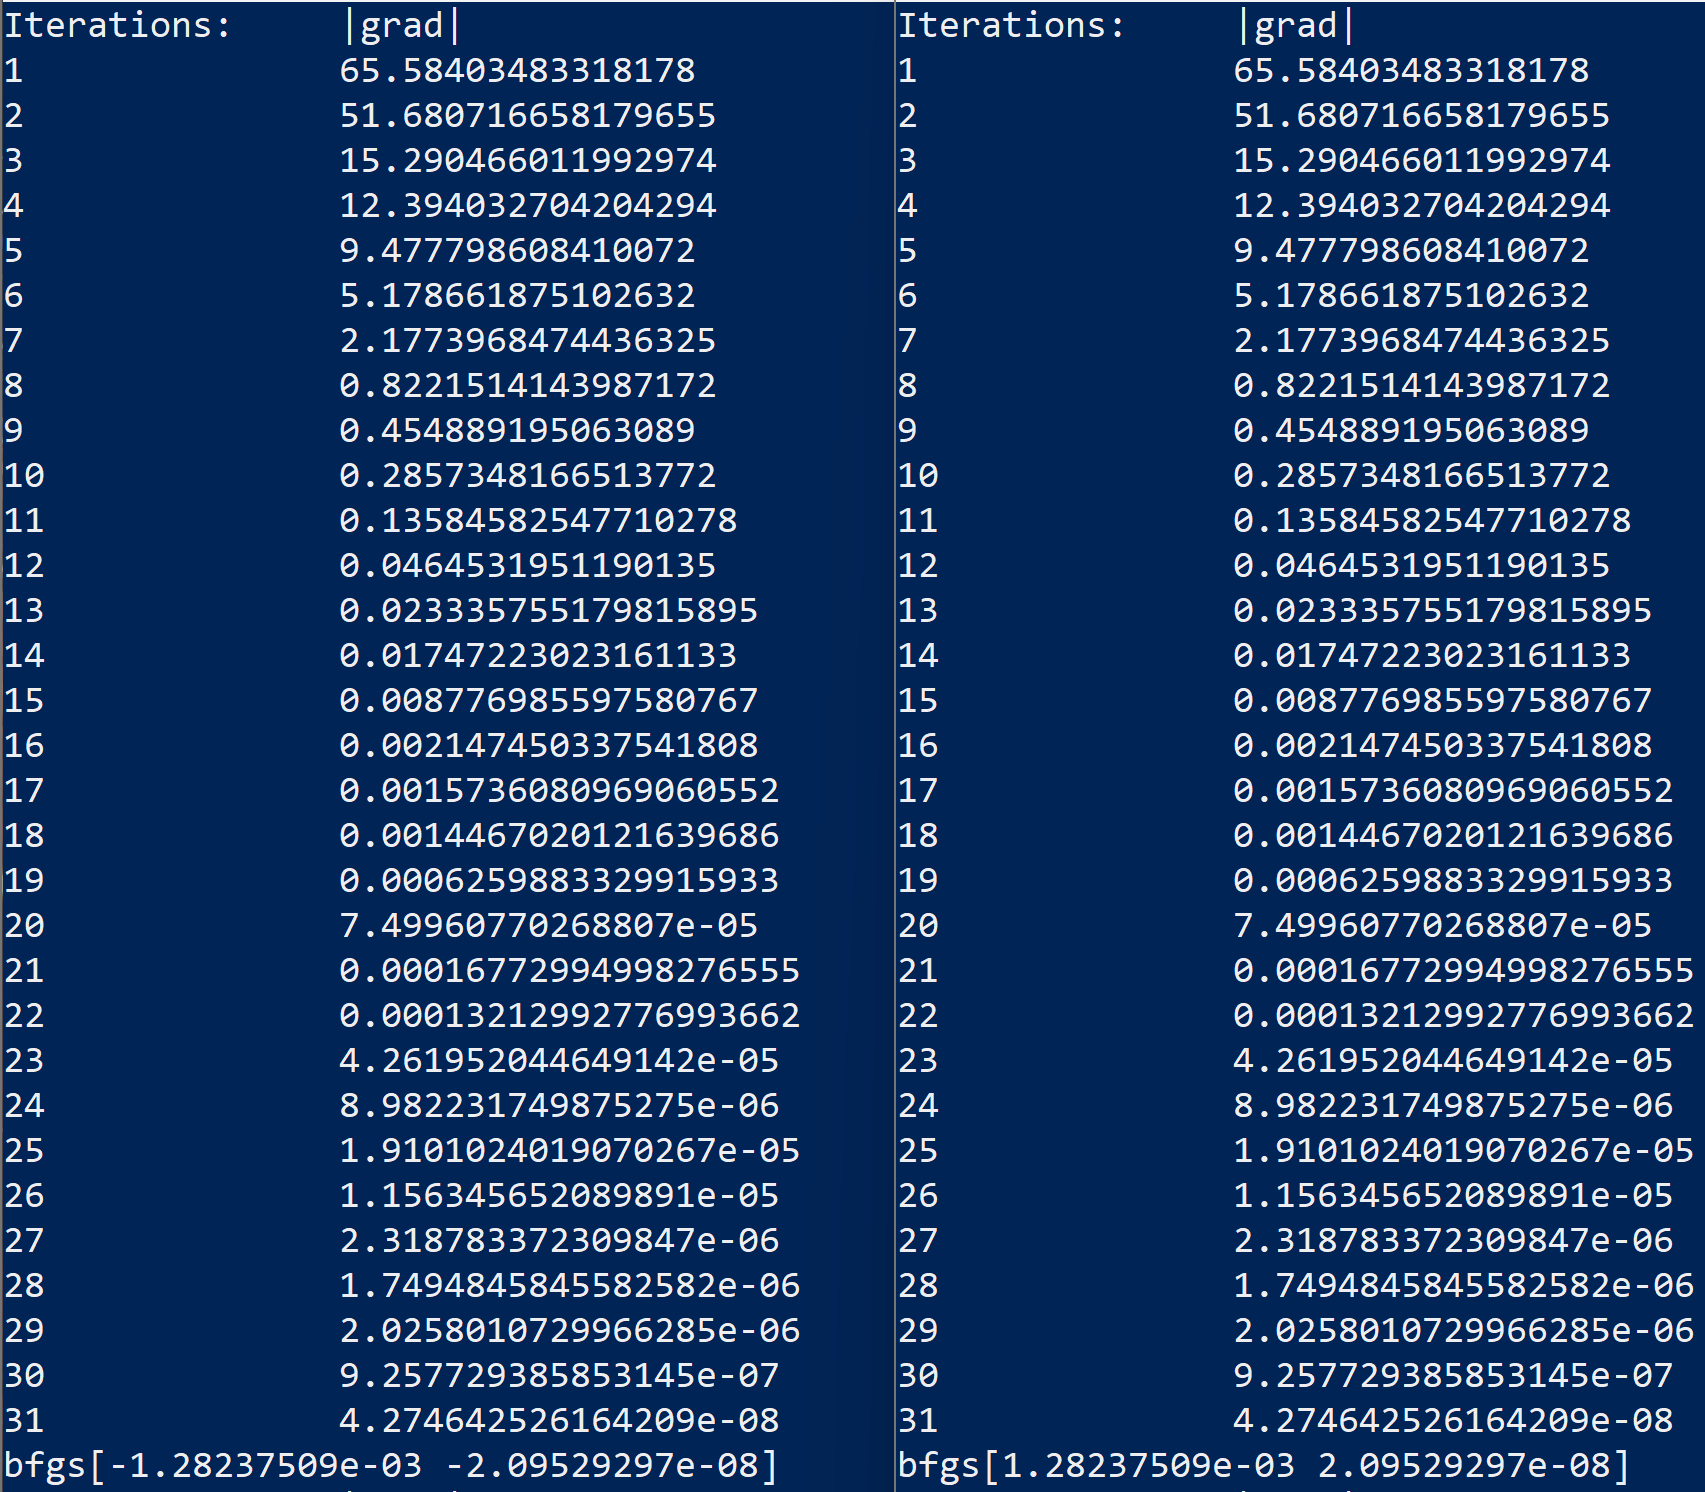
\includegraphics[width=0.75\linewidth]{d2.png}
    \caption{Function output for two dimensional Rosenbrock Function from one starting point}
    \label{fig:rosbrock}
\end{figure}
\newpage
\subsubsection{Two Dimentional Polynomial with Multiple Minima}
\label{sec:twodpolymult}
\begin{figure}[!ht]
    \centering
   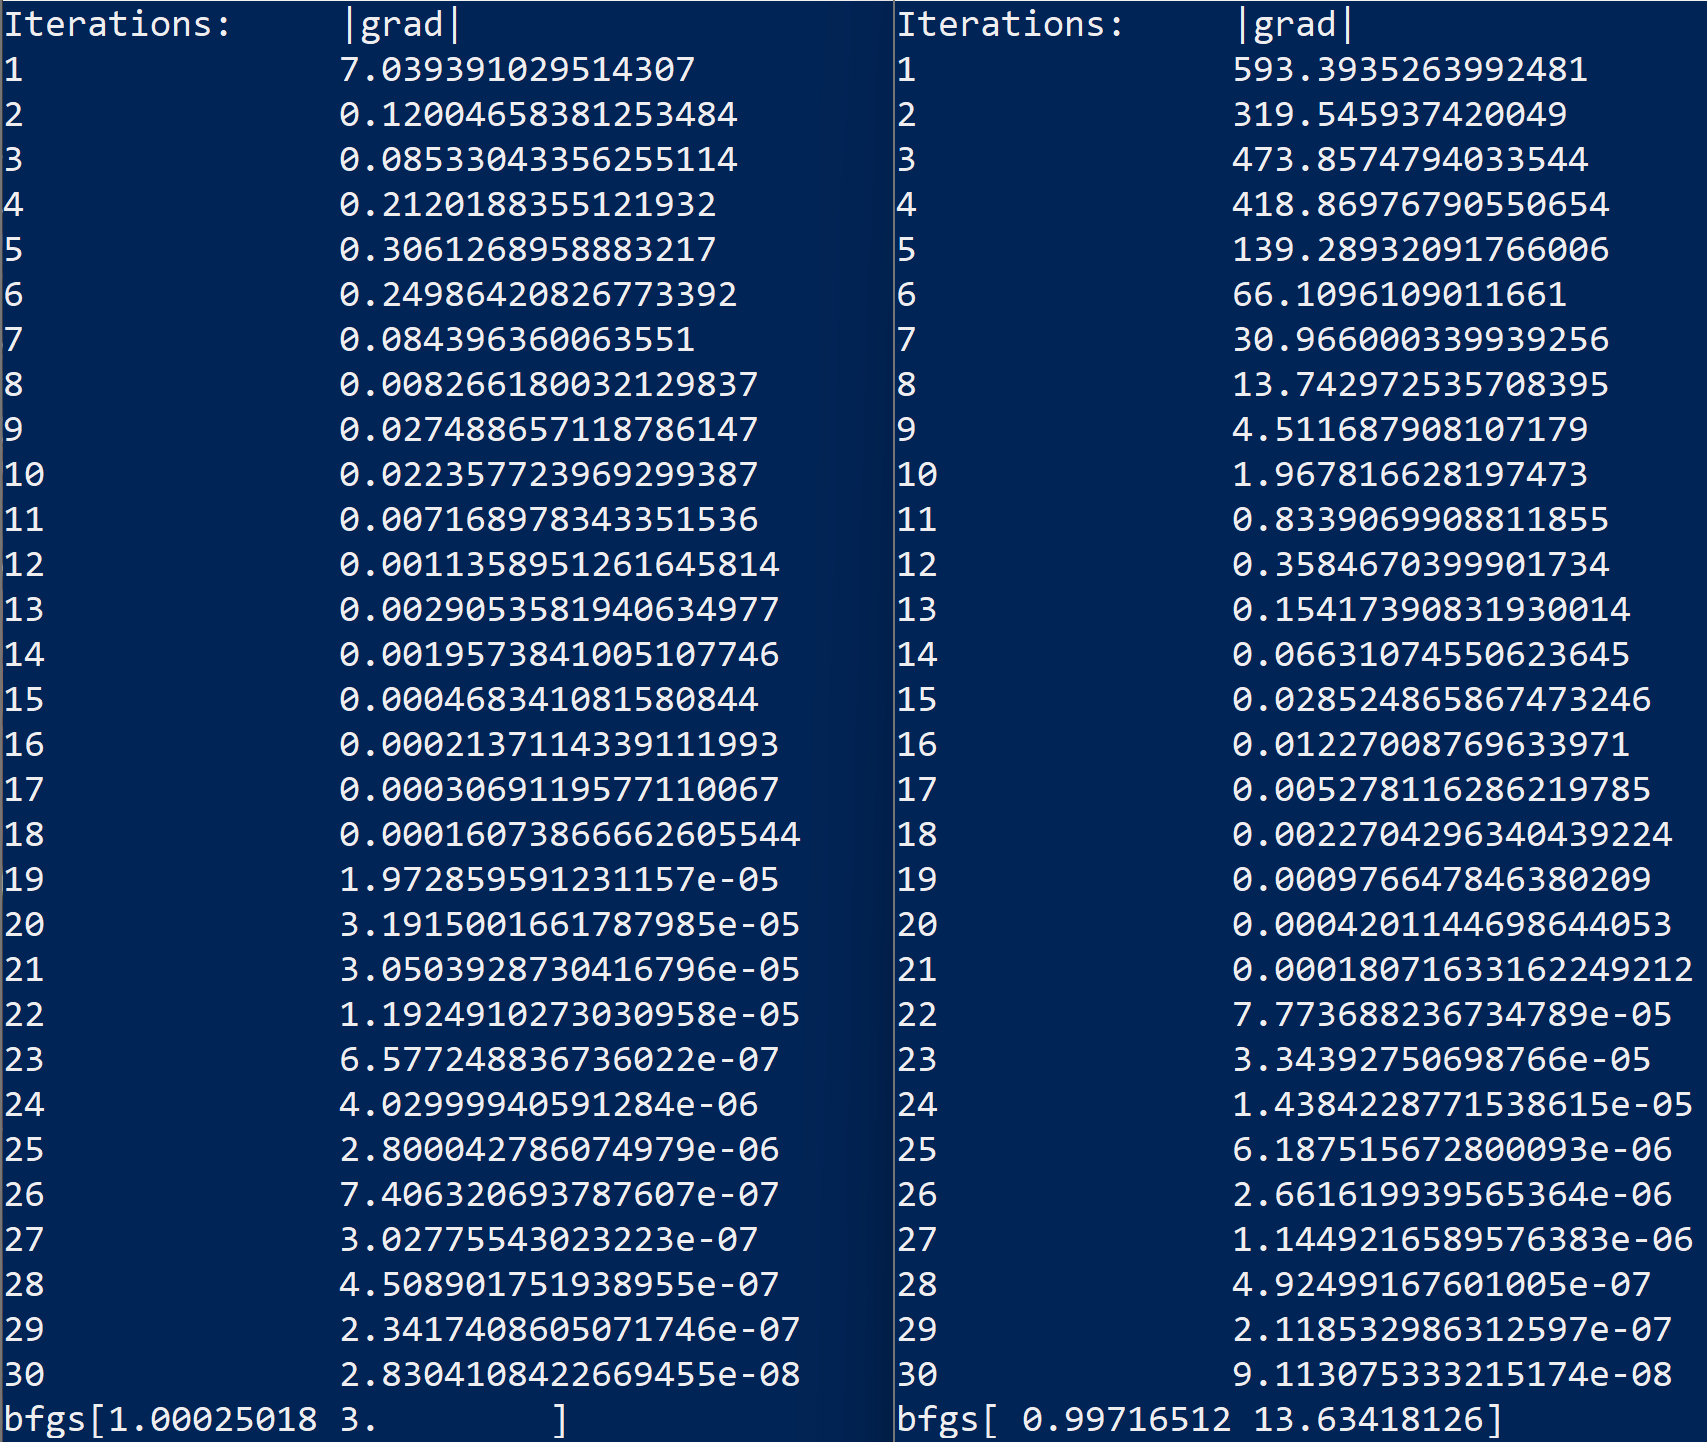
\includegraphics[width=0.75\linewidth]{d2mult.png}
    \caption{Function output for two dimensional polynomial from two starting points}
    \label{fig:d2mult}
\end{figure}
\newpage
\subsubsection{Three Dimentional Polynomial}
\label{sec:threedpoly}
\begin{figure}[!ht]
    \centering
   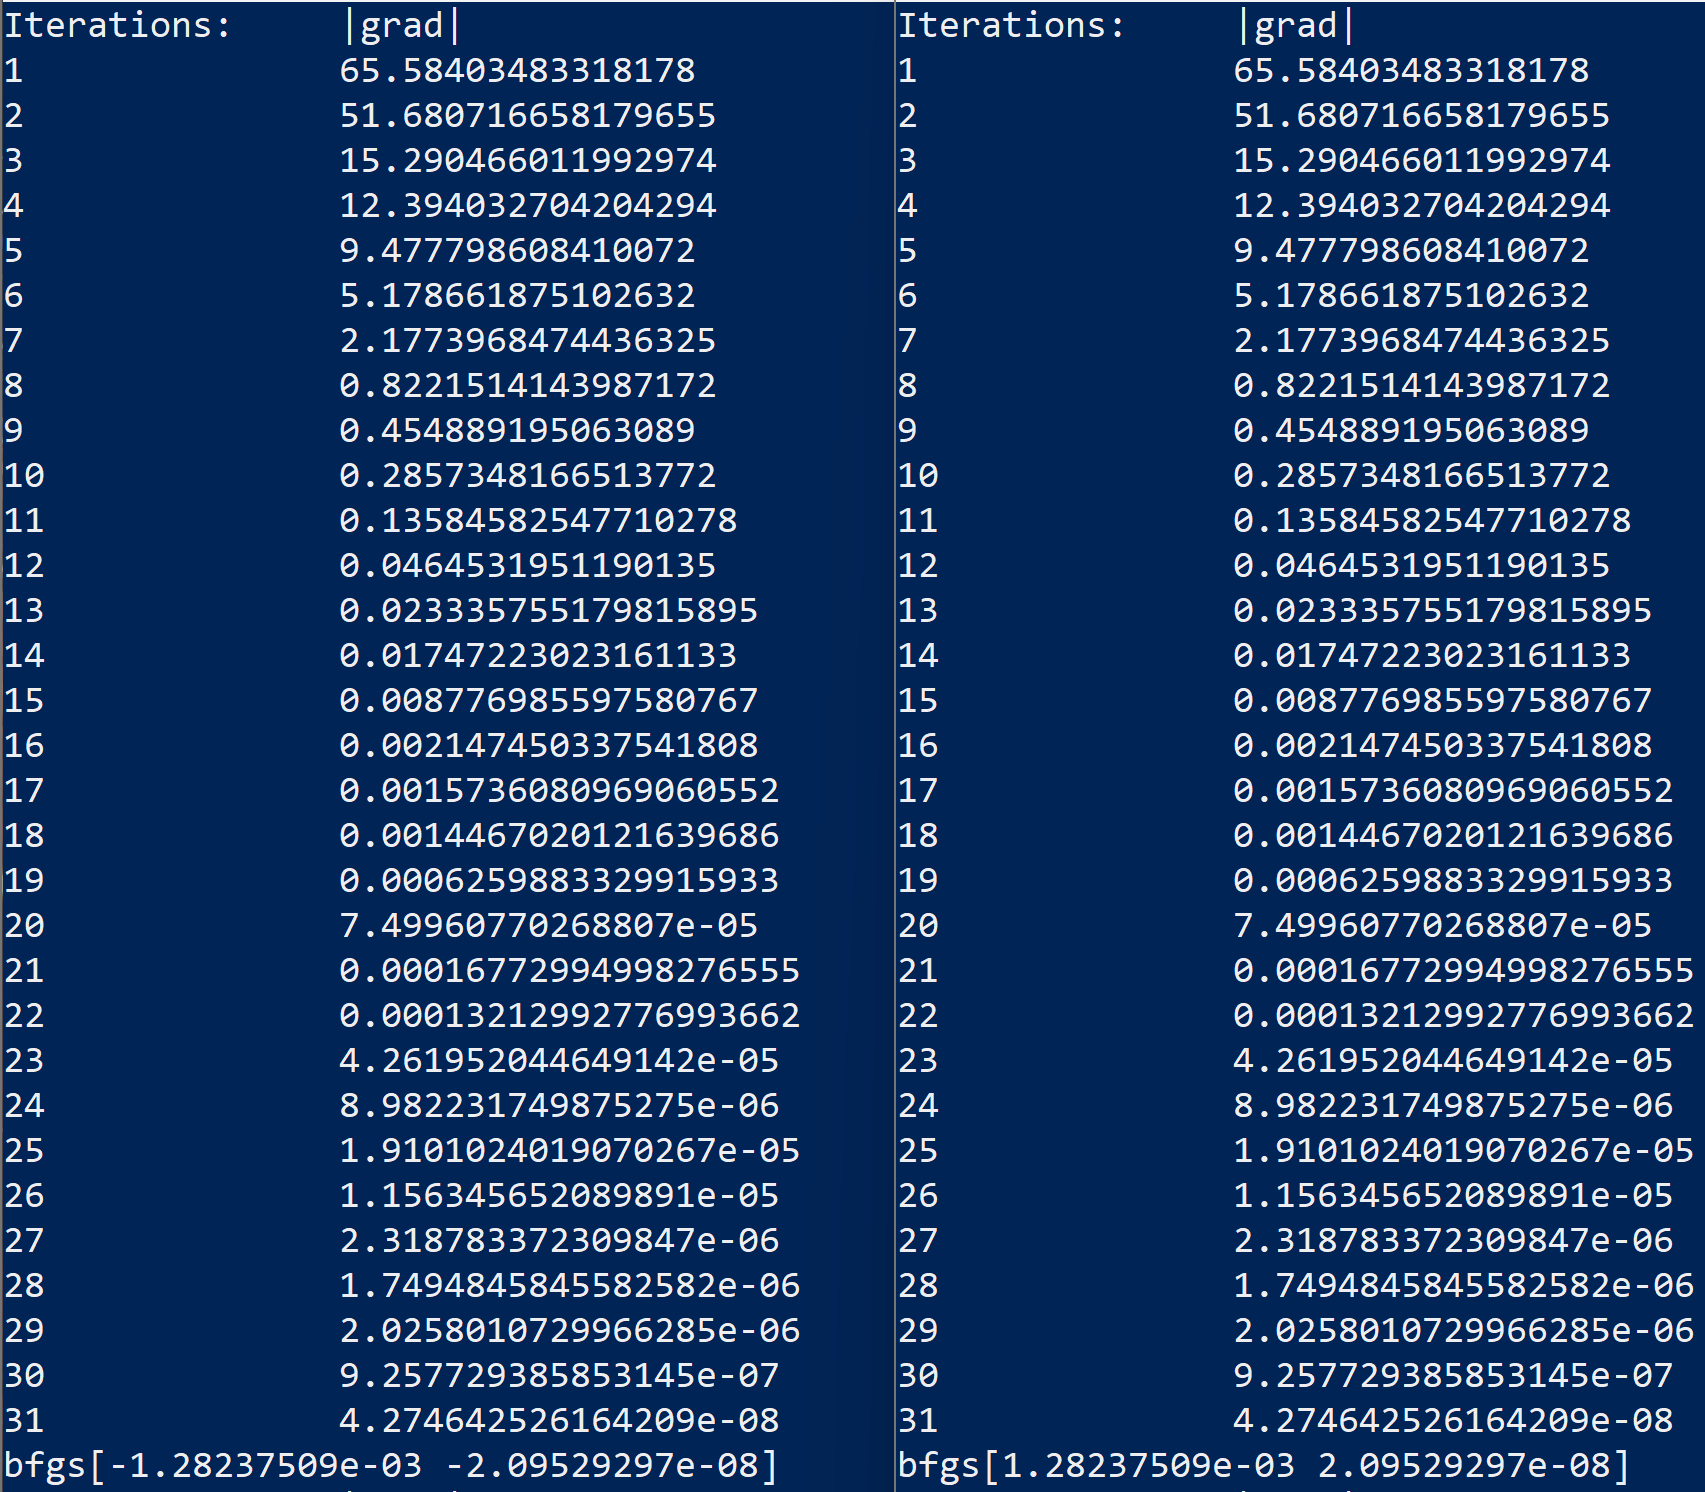
\includegraphics[width=0.75\linewidth]{d2.png}
    \caption{Function output for three dimensional polynomial from two starting points}
    \label{fig:d3}
\end{figure}
\newpage
\lstset{language=Python,%
    %basicstyle=\color{red},
    breaklines=true,%
    morekeywords={matlab2tikz},
    keywordstyle=\color{blue},%
    morekeywords=[2]{1}, keywordstyle=[2]{\color{black}},
    identifierstyle=\color{black},%
    stringstyle=\color{mylilas},
    commentstyle=\color{mygreen},%
    showstringspaces=false,%without this there will be a symbol in the places where there is a space
    numbers=left,%
    numberstyle={\tiny \color{black}},% size of the numbers
    numbersep=9pt, % this defines how far the numbers are from the text
    emph=[1]{for,end,break},emphstyle=[1]\color{red}, %some words to emphasise
    %emph=[2]{word1,word2}, emphstyle=[2]{style},    
}
\subsection{Code}

\subsubsection{BFGS Algorithm}
\label{sec:bfgs}
\lstinputlisting{ndofinal/bfgs.py}
\newpage
\subsubsection{Line Search Algorithm}
\label{sec:linesearch}
\lstinputlisting{ndofinal/lineSearch.py}
\newpage
\subsubsection{Zoom algorithm}
\label{sec:zoom}
\lstinputlisting{ndofinal/zoom.py}


\end{document}